\documentclass[a4paper]{article}

\usepackage{fullpage} % Package to use full page
\usepackage{parskip} % Package to tweak paragraph skipping
\usepackage{tikz} % Package for drawing
\usepackage{amsmath}
\usepackage{hyperref}
\usepackage[onehalfspacing]{setspace}
\usepackage{kotex}


\title{How to use the utility Git}
\author{20153334 전은영}
\date{2018.09.19}

\begin{document}
	
	\maketitle
	
	\section{소개}
	
	Git은 컴퓨터 파일의 변경사항을 추적하고 여러 명의 사용자들 간에 해당 파일들의 작업을 조율하기 위한 \textbf{'분산 버전 관리 시스템'}이다.
	
	예를 들어, 프로그래밍 프로젝트를 생각해보자. 처음부터 한 번에 완전한 결과를 만들 수 없다. 생각지 못한 문제가 생겨 코드를 수정하며 다양한 방법을 시도했지만 다 실패하고 원래대로 돌아가고 싶을 때 어떻게 해야할까? 다른 이름의 파일로 저장할 수도 있고, 이메일(원격 저장소)에 원본 파일을 저장하는 방안도 있다. 만약 잘 해결이 되었다고 하자. 팀 프로젝트라면 팀원들 모두에게 바뀐 부분 설명과 바뀐 파일을 메일로 보내야 할 것이다.위 방법들이 간단하지만 너무나도 귀찮고 효율적이지 않다. Git은 효율적인 버전 관리가 가능하도록 한다.
	
	버전 관리를 하려면 우리가 작업하는 실제 '로컬 저장소'와 '원격 저장소' 2가지가 필요하다. Git은 이 두 저장소를 연결하는 다리 역할을 맡고 있다.
	로컬 저장소로 작업하고 git으로 변경내용을 커밋 메시지에 담아 \textbf{push}를 하면 (충돌상황이 없다는 가정하에) 바로 원격 저장소에 변경 내용이 적용된다. 코드가 추가 되었으면 +로, 삭제되었으면 -로 수정된 부분만 시각적으로 볼 수 있다. 협업을 할 때 수정 내용을 일일이 메일로 보내야하는 번거로움도 없어진다. 또 원격 저장소의 업데이트 된 내용을 \textbf{pull}로 간편하게 로컬 저장소에 가져올 수 있다. 
	가장 핵심 기능은 충돌 사항을 체크해 주는 것이다. 팀원들이 같은 파일을 동시에 수정하고 push 한 경우 충돌이 발생했다는 것을 알려주고 책임자가 허락할 때까지(\textbf{merge}) 원격 저장소의 내용이 바뀌지 않는다.
	
	
	
	\section{Windows 10 설치 및 설정}
	
	
	\begin{enumerate}
		
		\item \textbf{https://git-scm.com/downloads} 사이트 접속. windows 클릭
		
		\begin{figure}[htbp]
			\begin{center}
				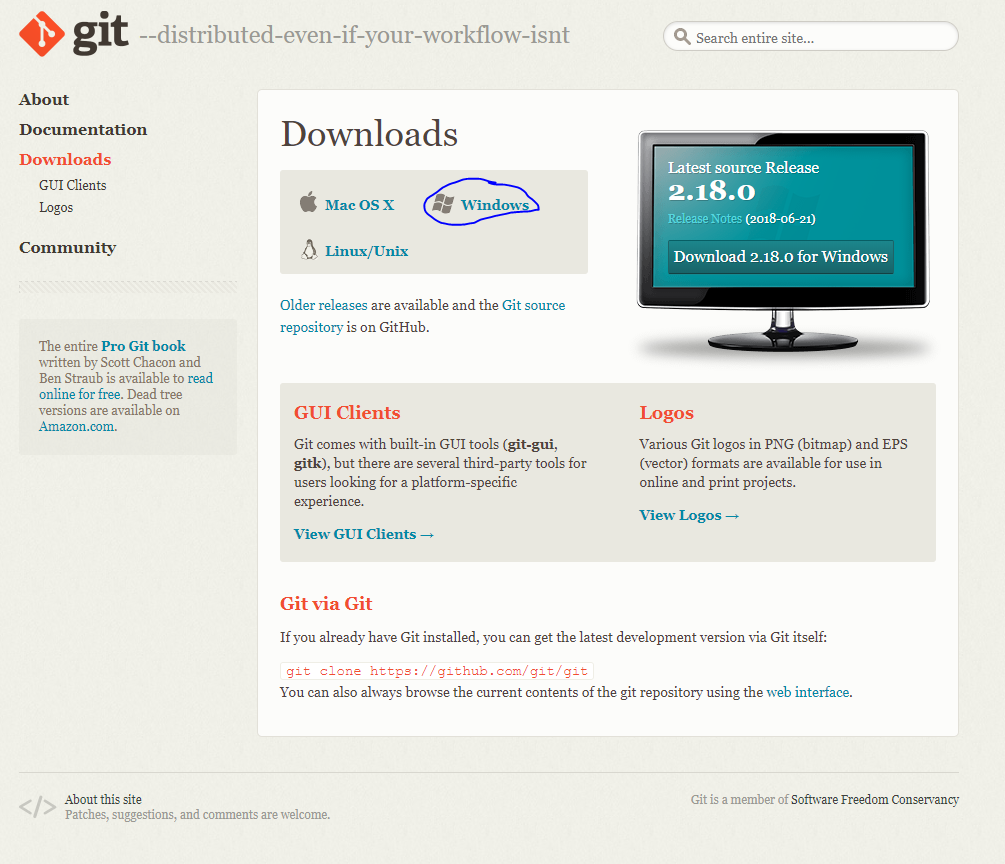
\includegraphics[scale=0.247]{source/install1}
			\end{center}
		\end{figure}
		
		
		
		* 바로 설치되지 않을 시, \textbf{'click here ...'} 부분을 클릭
		
		
		\begin{figure}[htbp]
			\begin{center}
				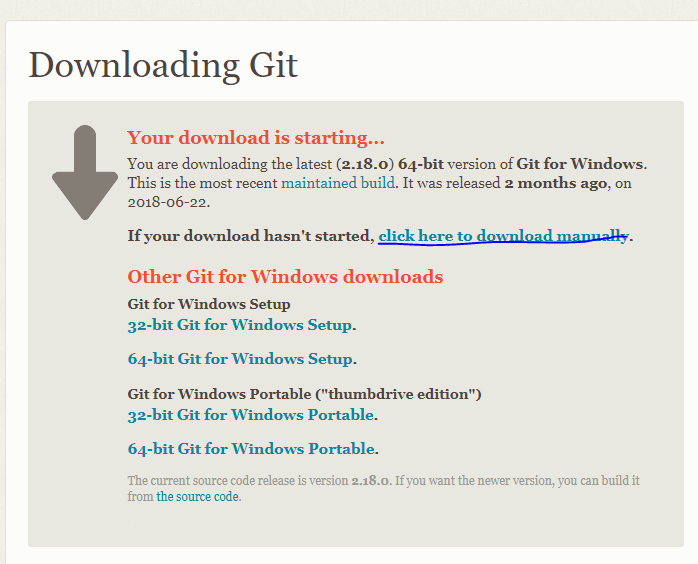
\includegraphics[scale=0.4]{source/install2}
			\end{center}
		\end{figure}
		
		
		
		\item installer에 하라는 대로 next next ...
		
		\begin{figure}[htbp]
			\begin{center}
				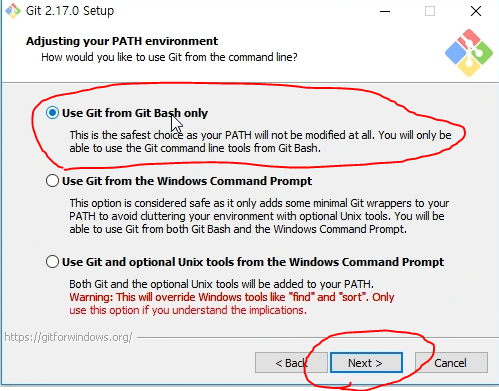
\includegraphics[scale=0.5]{source/gitbashonly}
			\end{center}
		\end{figure}
		
		
		windows 명령창에도 git 명령으를 쓰겠다는 것이 default다.
		
		본인은 git bash에서만 git 명령어 쓸 것이기 때문에 git bash only 선택\\
		
		
		
		\item 사용자 정보 설정
		
		* git bash 켜서 다음 명령어로 사용자 정보 설정
		
		\begin{verbatim}
		git config --global user.name "github 유저 네임"
		git config --global user.email "github 이메일 주소"
		\end{verbatim}
		* 설정되었는지 확인
		
		\begin{verbatim}
		git config --list
		\end{verbatim}
		
		
		
	\end{enumerate}
	
	
	\newpage
	
	\section{사용법}
	
	원격 저장소로 Github를 이용한다.
	
	\begin{enumerate}
		
		\item Github에 repository를 만든다.
		
		\item 우측 상단의 clone or download를 누르고 나오는 주소를 복사한다.
		
		\begin{figure}[htbp]
			\begin{center}
				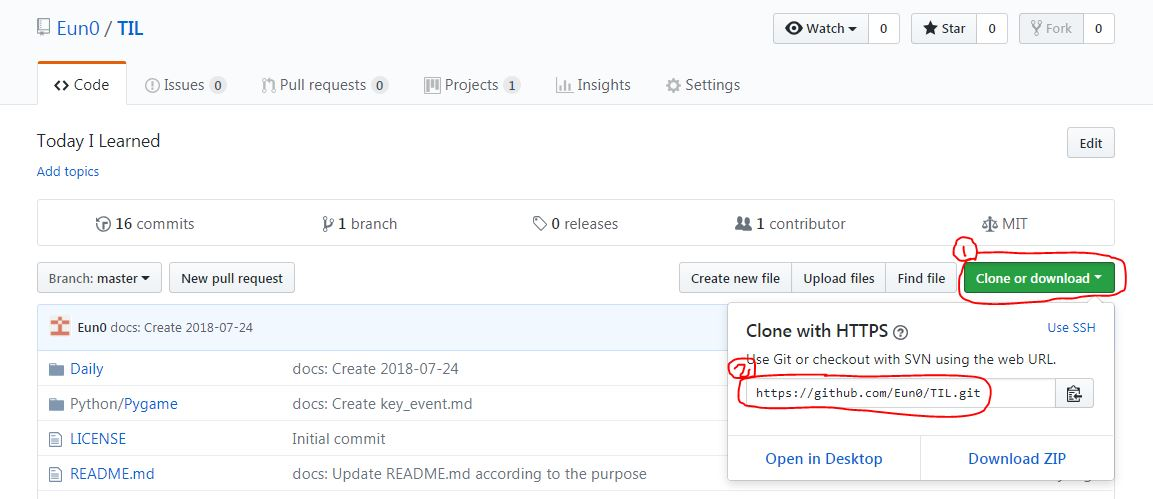
\includegraphics[scale=0.4]{source/cl1}
			\end{center}
		\end{figure}
		
		\item git bash를 키고 repository를 관리하고 싶은 위치로 가서 (cd 폴더이름 이용)
		
		
		
		\begin{verbatim}
		git clone 복사한 주소
		\end{verbatim}	
		
		
		\item 로컬에서 작업하기
		
		pull - \textgreater\, 작업 - \textgreater\, add - \textgreater\, commit - \textgreater\, push
		
		\begin{itemize}
			\item git pull : 원격 저장소의 변경된 부분을 로컬 저장소로 가져온다
			\item git add 파일 : commit할 파일을 add
			
			* 폴더 내 모든 파일 add
			
			\begin{verbatim}
			git add *
			\end{verbatim}
			
			* add 상태 확인
			
			\begin{verbatim}
			git status
			\end{verbatim}
			
			* add 안된 것은 
			\begin{verbatim}
			git add -u
			\end{verbatim}
			
			
			\item git commit -m "커밋메시지" : 커밋메시지로 commit
			\item git push (로그인 필요) : 충돌이 없다면 원격 저장소로 commit 내용을 보낸다.
			
			\item git reset --hard 커밋아이디 : 커밋마다 고유의 아이디가 있고, 그 커밋아이디 때로 돌아가는 명령어다.
		\end{itemize}
		
		
		
		
	\end{enumerate}
	
	
	\newpage
	\section{예제: 로컬의 assignment01.tex 파일 Github에 올리기}
	
	\begin{enumerate}
		\item Git bash 키고 clone한 디렉토리로 가서 git pull (원격 저장소의 변경 사항이 있을 수 있음)
		\begin{figure}[htbp]
			\begin{center}
				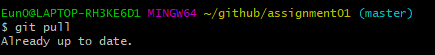
\includegraphics[scale=0.8]{source/1}
			\end{center}
		\end{figure}\\
		\item 원하는 작업을 한다. 2018\textunderscore09\textunderscore19.md 파일을 만들었다.
		\begin{figure}[htbp]
			\begin{center}
				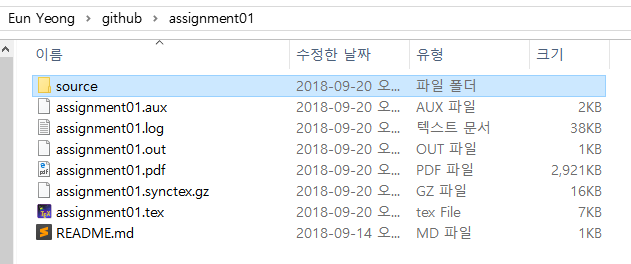
\includegraphics[scale=0.8]{source/2}
			\end{center}
		\end{figure}\\
		\item Git bash에서 git add 2018\textunderscore09\textunderscore19.md (git status로 확인)
		\begin{figure}[htbp]
			\begin{center}
				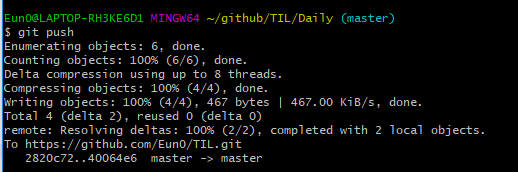
\includegraphics[scale=0.8]{source/6}
			\end{center}
		\end{figure}
		\newpage
		\item git commit -m "Create 2018\textunderscore09\textunderscore19.md"
		\begin{figure}[htbp]
			\begin{center}
				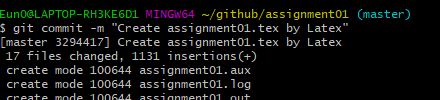
\includegraphics[scale=0.8]{source/4}
			\end{center}
		\end{figure}
		\item git push
		\begin{figure}[htbp]
			\begin{center}
				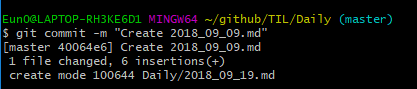
\includegraphics[scale=0.8]{source/5}
			\end{center}
		\end{figure}
		\item Github에서 확인
		\begin{figure}[htbp]
			\begin{center}
				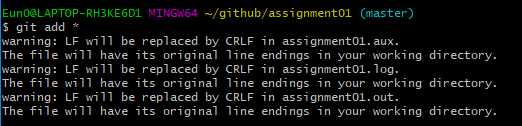
\includegraphics[scale=0.8]{source/3}
			\end{center}
		\end{figure}
		
	\end{enumerate}
	
	
	
	
	
	
	
	
	
	
	
	
	\bibliographystyle{plain}
	
\end{document}
